\documentclass[sigconf]{acmart}

\usepackage{booktabs} % For formal tables

\usepackage{proof}
\usepackage{graphicx}

% Copyright
%\setcopyright{none}
%\setcopyright{acmcopyright}
%\setcopyright{acmlicensed}
% \setcopyright{rightsretained}
%\setcopyright{usgov}
%\setcopyright{usgovmixed}
%\setcopyright{cagov}
%\setcopyright{cagovmixed}


% DOI
% \acmDOI{10.475/123_4}

% ISBN
% \acmISBN{123-4567-24-567/08/06}

%Conference
% \acmConference[WOODSTOCK'97]{ACM Woodstock conference}{July 1997}{El
%  Paso, Texas USA} 
% \acmYear{1997}
% \copyrightyear{2016}

% \acmPrice{15.00}


\begin{document}
\title{Languages of Play}
\subtitle{Towards semantic foundations for game interfaces}


%% Double blind review
% \author{Chris Martens}
% \affiliation{%
%   \institution{North Carolina State University}
%   \city{Raleigh} 
%   \state{NC} 
% }
% \email{martens@csc.ncsu.edu}
% 
% \author{Matthew Hammer}
% \affiliation{%
%   \institution{University of Colorado, Boulder}
%   \city{Boulder}
%   \state{CO}
% }
% \email{XXX@XXX.edu}


\begin{abstract}
Abstract goes here. A full paper's maximum length is 10 pages; a short
paper's is 6 pages. Track: probably Game Design and Development.
\end{abstract}


\keywords{games, programming languages, formal methods}

\maketitle

\section{Introduction}

To study how players interact with games, we examine both the rules of the
underlying system and the choices made by the player. One recognizes the
value in constructing detailed models of player cognition: while a game as
a self-contained entity can allow us to learn about its mechanics and
properties as a formal system, we cannot understand the {\em dynamics} of
that system unless we also account for the human half of the equation.

% \begin{figure}
% 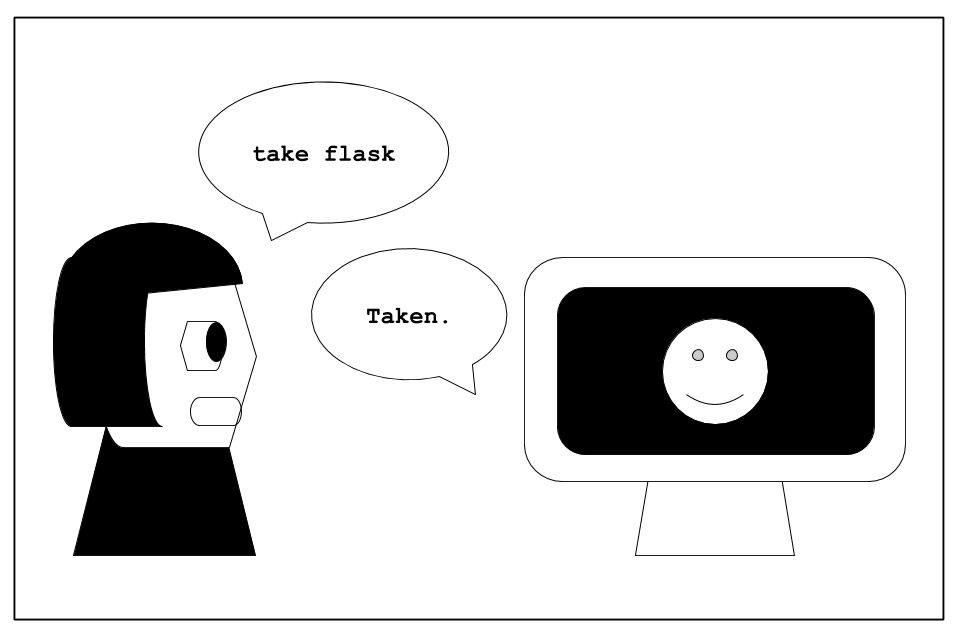
\includegraphics[width=0.4\textwidth]{conversation.png}
% \caption{The observable features of a game loop: a player and a game in conversation.}
% \end{figure}

What often goes missing in such a discussion, however, is the {\em
interface} between the two. Crawford~\cite{crawford2003chris} defined
interactivity in games as their ability to carry out a conversation with a
player, including listening, processing, and responding, identifying the
importance of all three to the overall experience. Cardona-Rivera and
Young~\cite{cardona2014games} later proposed a more detailed conceptual
framework following the slogan {\em games as conversation}, providing
grounded evidence for the communicative strategies of games following
conventions in line with cognitive theories for human-to-human
conversational understanding, such as Grice's maxims (XXX cite).

Just as the field of film studies has developed a notion of {\em
vocabulary} that visual storytellers use to communicate with audiences,
such as the cinematic device of {\em intercutting} used to convey
simultaneous action,
scholars have studied the vocabulary and representational conventions of
games (XXX cite something re games literacy? salen and zimmerman?) that
designers employ to communicate with players, such a horizontal green bar
floating above an avatar representing its health or a question mark
labeling an object as a reward or power-up. In interactive media, we also
adopt the notion of {\em affordances} in terms of what kinds of actions
these representations invite: a health bar above an avatar suggests it may
be attacked, whereas a question mark labeling a box suggests it might be
opened.
% Designers term these representational conventions taken as a
% systemic whole a {\em design language} (XXX cite?) 
%
We have recognized that a symbolic, discretized and representational
approach to looking at these design decisions has value: the term {\em
design language} (XXX cite) indicates a recognition that these symbols and
affordances operate together as a system.

However, play is a two-way street. Design language explains how the computational half of
the conversation expresses itself to the human half. This paper introduces
an account of how the human half of the game loop expresses themselves to
the computational half.

The paper introducing the Game Ontology Project~\cite{zagal2007towards} asserts,
\begin{quote} \em
The interface is where the player and game meet, the mapping
between the embodied reactions of the player and the manipulation of game
entities. It refers to both how the player interacts with the game and how
the game communicates to the player.
\end{quote}
The authors subdivide interface into {\em input} and {\em presentation},
where presentation includes the representational strategies already
discussed. {\em Input} is further subdivided into {\em input device} and
{\em input method}, where input devices are hardware controllers (mice,
keyboards, joysticks, etc.) and input {\em methods} start to brush the
surface of something more semantic, analogous to a design language: it
includes choices about {\em locus of manipulation} (which game entities can
the player control?) and direct versus indirect action, such as selecting
an action from a menu of options (indirect) versus pressing an arrow key to
move an avatar (direct).


\begin{figure*}
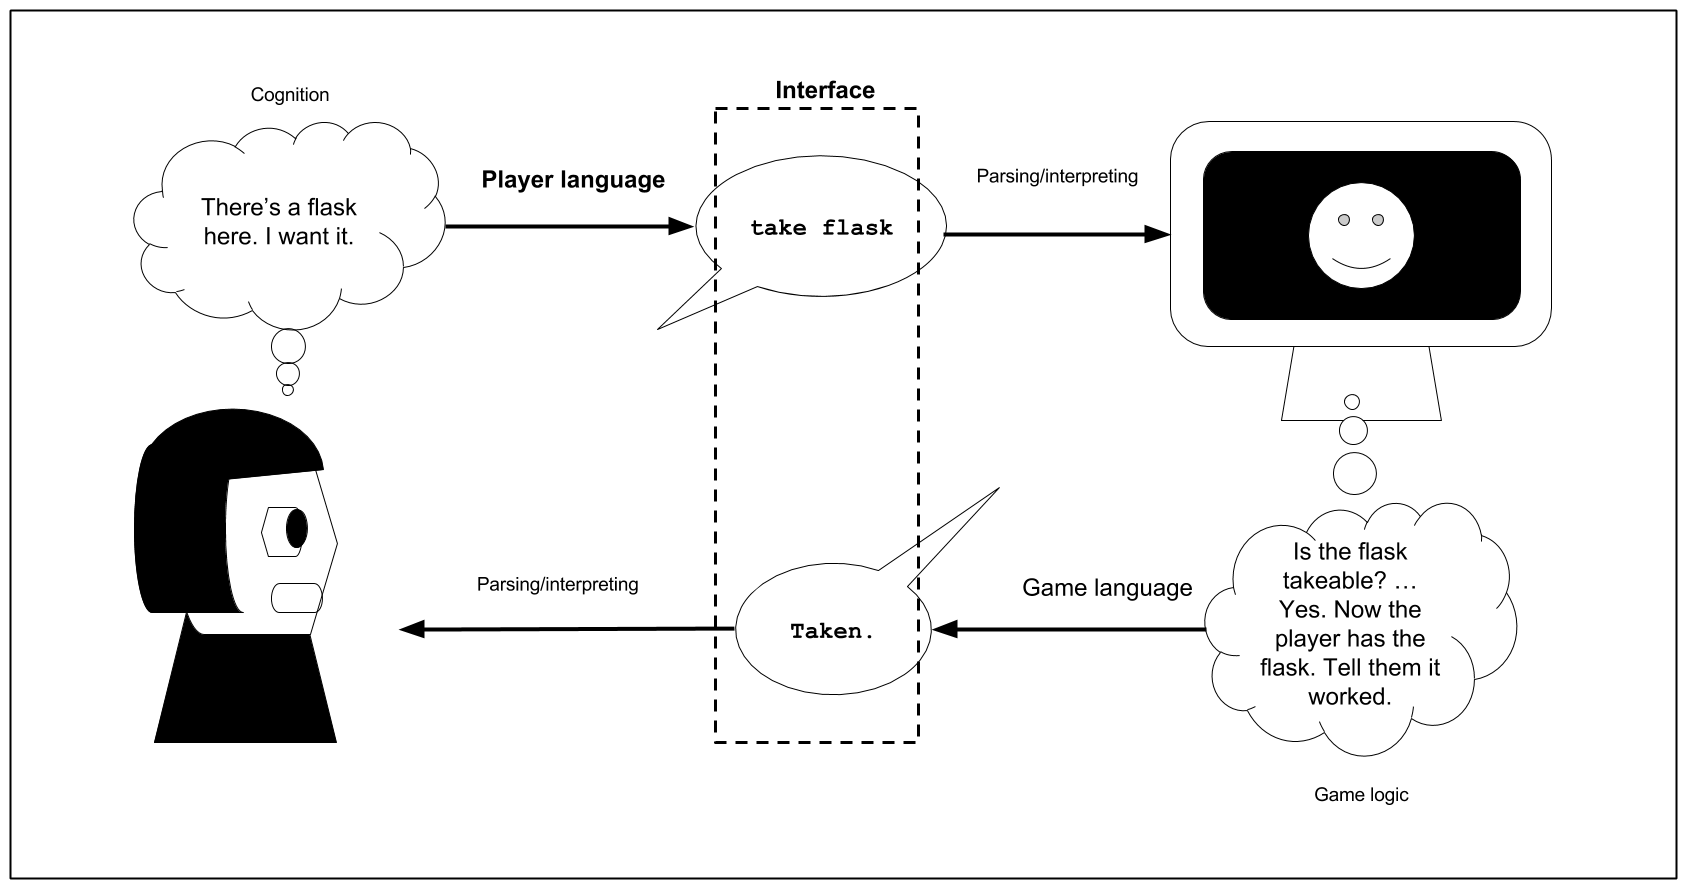
\includegraphics[width=0.75\textwidth]{conversation-processing.png}
\caption{A process diagram of a game loop: player and game conversation as
it relates to language, interface, and cognition.}
\end{figure*}

(XXX this is kind of a description of the figure)
play is a two-way street: a game provides affordances for action, a player
takes action based on those affordances, and the game responds in turn with
feedback that develops the player's mental model for the behavior of the system
implied by the interaction as a whole. And, 

How does the player communicate their intent, and how does a
digital game recognize this intent?

Clearly they use some kind of language, but since the constraints on what
language they may use are wholly determined by a piece of software (the
game interface), we argue that this language has more in common with a {\em
programming language} (loosely defined as a formal language whose meaning
is fully grounded in a computational system) than a natural language. We
argue that conceptualzing player communication in terms of hardware
interactions (button presses, mouse clicks) is too {\em low-level} of an
approach to meaningfully study interaction, and that instead we should make
sense of these interactions on a {\em per-game} basis in terms of the {\em
meaning} with which a game imbues these interactions. 

Accordingly, each game provides a player with a unique formal language,
termed ``programming language'' (though it may have a great deal in common
with other games' languages) to express themselves. While some researchers
have recognized interaction vocabularies common to certain types of games,
their conclusion was to codify these conventions as a {\em single}
programming language (VGDL, XXX cite), misleadingly positioned as though it
could represent all (or a broad category) of games in a high-level way.
We suggest that instead, the landscape of game representations and player
affordances is as varied as the landscape of programming languages, and an
adequate computational framework should be one that can accommodate the
encoding of many such languages, such as a {\em logical framework} (XXX
cite Twelf or something).

What is to be gained by the game-interfaces-as-programming languages analogy?

The programming languages (PL) community has a long and deep history of
assigning mathematically formal semantics to languages and analyzing those
semantics. As games researchers become more interested in the emergent
consequences of the systems they assemble, the tools of PL theory have a
lot to offer. For example, PL theory provides an account of how to relate
meaning in a {\em low level} representation (such as assembly language, or
on the games side, hardware-level interactions) to meaning in a {\em
high-level} language (such as a language like Java or a game's state
space), allowing us to draw abstraction boundaries and consider system
components in compositional terms. For example, we can consider what it
means to have a game with the same {\em internal mechanics} (or what Salen
and Zimmerman (XXX) call {\em constiutative rules}) but distinct interface,
comparing the meaning of these interfaces on formal terms.

% In Salen and Zimmerman (XXX cite) terms,
% PL theory can help us formalize the {\em constituative mechanics} of a
% game's interface so that we may consider distinct {\em operational rules} 
% that interface with them. 

% XXX example: parser vs. hypertext interactive fiction?
%
% Parser:
%   Interface:
%     >
%   Recognized utterances - contextual:
%    > <verb> <noun>
%    > <verb>
%    > <verb> <noun> <preposition> <noun>
%
% Hypertext:
%   Interface: contextual, e.g.
%     [[go north]] or [[go south]] or [[take sword]] ?
%   Recognized utterances:
%     (link clicks) - 1 dimensional, contextual, ambiguous


Furthermore, by considering a player's language of expression as an object
of study in its own right, we center her as a co-designer of the experience
afforded by a game. When we treat a player's interactions as not simply an
arbitrary sequence of button presses that advances and reveals the
designer's intent, but instead as its own distinct {\em voice} that a game
system must listen and respond to, we enable the player to {\em co-create}
with the system, potentially developing stronger systems thinking skills in
the player, eliciting deeper understanding and even deeper emotional
investment.

In the remainder of the paper, we concretize the analogy by introducing the
components of a theoretical account of a programming language (syntax, type
system, and operational semantics) and its analog in a game. We walk
through an example to illustrate how to think about a game in terms of its
language-like affordances, and we demonstrate the payoff of this line of
thought by extending the metaphor to account for {\em player skills} as
``programs,'' effectively representing mental models for how to accomplish
some task in terms of the game's linguistic constructs.

\section{Related Work}

AI action languages (planning, event calc, etc.); general game AI frameworks

FRP? Other PL stuff; embedded DSLs?

PlaySpecs

Hazel

\section{A Framework}

  % (that table from the doc should go here)

  % Background: Syntax, type systems, and operational semantics

  In the formal study of a programming langugage, one may define a language
  in three parts: syntax, type system, and operational semantics.
  \begin{itemize}
    \item The {\em syntax} is written in the form of a (usually)
      context-free grammar describing the allowable expressions.
    \item A {\em type system} further refines the set of allowable
      expressions into a set of {\em meaningful} expressions, and provides
      a mapping between an expression and an approximation of its meaning.
      Type systems are usually designed in conjunction with the operational
      semantics to have the property that {\em well-typed programs don't go
      wrong}, i.e., every expression assigned a meaning by the type system
      should have a well-defined runtime behavior.
    \item An {\em operational semantics} defines how runnable programs
      (e.g. a function applied to an argument) {\em reduce} to values. This
      part of the definition describes how actual computation takes place
      when programs in the language are run. It is important to note that
      the operational semantics need not reflect the actual {\em
      implementation} of the language, nor is it specific to a ``compiled''
      versus ``interpreted'' understanding of the language: it is simply a
      mathematical specification for how any compiler or interpreter for
      the language should behave.
  \end{itemize}
  
  Providing a formal language definition in programming languages research
  has several purposes. One is that it enables researchers to explore
  and prove formal properties of their language, such as {\em well-typed
  programs don't go wrong}, or in a language for concurrency, a property
  like deadlock freedom. However, an even more crucial advantage of a
  language specification is not mathematical rigor but human capacity to do
  science. A language definition is a {\em specification}, similar to an
  application programmer interface (API) or an IEEE standard: it describes
  an unambiguous interface to the language along an {\em abstraction
  boundary} that other human beings may access, understand, and implement,
  without knowing the internals of a language implementation.  It is a
  necessary component of reproducibility of research, and it allows
  researchers to build on each other's work. We believe that an embrace of
  the formal specification in games research can play a similarly important
  function.

  Having provided loose definitions of these terms, we now wish to draw out
  the analogy between a {\em language} specification and a {\em game}
  specification. To treat a game in this manner, we wish to consider player
  affordances and actions, as well as their behavior (mechanics) in the
  context of the game's running environment. We summarize the components of
  this correspondence in Table~\ref{tab:correspondence}.

  \begin{table}
  \begin{tabular}{ll}
    PL concept & Game concept\\
    \hline
    Syntax & Recognized player actions \\
    Type system & Meaningful player actions \\
    Operational semantics & Game mechanics \\
    Runtime store & Game world \\
    Normalized programs & Play traces 
  \end{tabular}
  \label{tab:correspondence}
  \end{table}

  (XXX turn into sentences)
  Running example: moving through a discrete set of rooms,
  acquiring objects placed in those rooms.

  \subsection{Player actions as syntax}

  Should be context free; recognizable by a parser; define well-formed
  expressions by the player
  
  Possibilities for movement:
  pressing a directional arrow;
  typing a direction;
  moving the mouse or joystick

  Possibilities for taking an item:
  pressing a designated button;
  typing ``\verb/take <item>/'';
  colliding with the item

  BNF for interface 1:\\
  \verb/move <dir> | collect/

  BNF for interface 2:\\
  \verb/go <dir> | take <thing>/\\
  n.b. larger set of allowable utterances; meaning is less contextual
  (easier to infer by itself what parts of the game state it will depend
  on)

  BNF for interface 3:\\
  \verb/move <dir>/\\
  n.b. much {\em more} contextual; it's impossible to infer what each
  action will ``do'' in the game and which parts of the game environment it
  depends on

  Additive vs. subtractive affordances:

  Just like with the rest of a game's rules, its language of play has both
  additive and subtractive properties: it provides the menu of options for
  what types of things are {\em permissible}, i.e. likely to result in
  meaningful interaction with the game system, but it also establishes
  which utterances are {\em disallowed}, i.e. that it is not meaningful to
  say ``take'' without providing an object to the command.

  ... is the grammar for a blank text field that or is it just any typed
  string, and the type system what enforces the grammatical structure?
  (XXX)

  \subsection{Structured affordances as type systems}
  
  Whether an utterance is {\em meaningful} or not will depend on
  the runtime game state, and is a distinct question from whether it is
  well-formed. For example, whether or not we can {\em take
  flask} depends on whether the flask is present, or indeed whether a {\em
  flask} is even a recognized game object. But unless ill-formed intents can be
  recognized a priori (such as: if we know the complete set of possible
  game objects ahead of time and can reject commands that refer to entities
  outside of that set), we must treat this command as well-formed {\em
  syntax} and relegate its failure to integrate with the runtime game
  environment to the {\em mechanics} (operational semantics).

  However, we can rule out an approximation of ill-formed utterances using
  type systems. For example, if we know the ...
  (only take portable things, only talk to characters, etc - could be
  specified at the grammar level)
  
  Providing the player with {\em only the option of saying} those
  utterances that ``make sense'' in this regard corresponds to a strong
  static type system: e.g. choice-based interface to parser-based
  commands...

  Consider fishing minigame in Stardew Valley: the player only has a way of
  {\em expressing} a ``reel in fishing line'' verb in the context of the
  fishing minigame. This action has no corresponding utterance in the main
  interface of the game.

  XXX analogy to structure editors, visual prog environments, discoverable
  choice-based interfaces...


  \subsection{Game environment as external runtime}

  To characterize mechanics, we will also need an account of expressions
  permissible in the game's language (e.g. display a room, make a sound,
  make an object disappear, etc. --- things more commonly accounted for in
  formal game description languages). 

  We will also need to characterize ``hidden'' state of the game...
  predicate syntax... locations of things, adjacency graph to describe the
  world map

  World state $\sigma$; game expressions $e_g$; used in the judgments
  defining operational semantics below


  \subsection{Mechanics as operational semantics}

  XXX - need to explain step syntax, as well as inference rules

  \newcommand{\stepsto}{\rightsquigarrow}

  Judgment: $\sigma; e_p \stepsto \sigma'; e_g$ \\
  where $e_p$ is a player expression and $e_g$ is a game expression, and
  $\sigma$ and $\sigma'$ are game states. This judgment should be read:
  ``Under state $\sigma$, the game responds to player action $e_p$ by
  changing to state $\sigma'$ and conveying information $e_g$.''

  Mechanics of interface 1:

  \[
    \infer{
      \sigma, at(R); PLAYER: move<dir> \stepsto \sigma, at(R'); GAME:
      display(R')
    }
    {
      indir(dir, R, R') \in \sigma
    }
  \]


  \[
    \infer{
      \sigma, at(R); PLAYER: move<dir> \stepsto 
      \sigma; GAME: \mathsf{fail\_feedback}
    }
    {
      indir(dir, R, R') \notin \sigma
    }
  \]

  XXX more rules

  n.b. this semantics is not really ``complete'' in the sense that it does
  not define meaning for sequences of actions, just single exchanges... how
  to compose actions?

  \subsection{Play traces as (normalized) programs}
  
  Argument for having a syntactically-well-founded structured term for a
  play trace

  \subsection{Theorems?}

  While it is not often considered of high priority for game designers to
  prove theorems about their software, and in fact a rich culture is
  enjoyed around the concept of {\em glitches} in games programs, a
  meticulous designer may still wish to understand the scope, complexity,
  and compatibility of her game approximated by compatibility between 
  player affordances and game rules. A formal examination of the game's
  properties, when studied as a programming language, can provide just
  that:

  Well-typed programs don't go wrong ~= every possible player utterance has
  a defined meaning within the game rules

  XXX example of this failing?
  
\section{Example}
To test the extent to which this analogy holds beyond a smallest example,
we attempt to describe the logic of a complex resource economy game with
an extensive player language. In {\em Stardew Valley} (XXX cite), the
player has an inventory that permits varied interactions with the world,
beginning a number of tools for farming (axe, hoe, scythe,
pickaxe) which do different things in contact with the resources in the
surrounding environment; most include extracting some resource (wood,
stone, fiber, and so on), which themselves enter the player's inventory and
can be used in further interaction with the game world. There are also
context-sensitive interactions between the player and non-player characters
(NPCs), interfaces through which new items may be purchased (shops), and
mini-games including fishing.

While a full account of the language that this game affords the player is
beyond the scope of this paper, what follows is an attempt to include a
representative sample of the actions and affordances found in this game,
presented in terms of the framework described above.

(XXX summarize what we are doing in this section)

\subsection{Syntax}

% move, apply tool, interact (open chests, talk to people, open doors,
% sleep)
% eating, giving things to npcs

(XXX concrete vs. abstract syntax analog to controls vs. player actions?)

\newcommand{\param}[1]{\langle #1 \rangle}
\newcommand{\syn}[1]{\mathsf{#1}}

(an item is something held, an entity is something in the world)
\begin{eqnarray*}
action &::=& \syn{select} \param{item}\\
       &\mid& \syn{apply} \param{entity}\\
       &\mid& \syn{inquire} \param{entity}\\
       &\mid& \syn{move\_near} \param{entity}\\
       &\mid& \syn{move\_offscreen} \param{direction}
\end{eqnarray*}

While it would be tempting to use the syntax layer to encode the kind of
higher-level actions performed in the game most frequently---tilling land,
planting seeds, conversing with NPCs---we want to accurately reflect the
{\em extensibility} of Stardew Valley's player language by describing the
general system from which these actions are derived. In other words, rather
than having each instance of such an action be a special case that a player
must learn how to speak as an independent vocabulary term, instead, they
learn it through {\em composing} the pre-existing constructs of selecting items
and applying them to objects in the world. For example: (XXX explain this
more)

Higher-level actions:
\begin{verbatim}
action hoe = select hoe; move_near shrub; apply shrub
action mine = select pickaxe; move_near rock; apply rock
action enter_shop = move_near shop; inquire door(shop)
action talk = move_near npc; inquire npc
action plant = select seeds; move_near tilled_ground; apply tilled_ground
\end{verbatim}

\subsection{Context Dependence}

include discussion of whether the above sequences of actions will actually
succeed or not; protocols...

include discussion of inventory menu, shops, crafting, recipes, other contextual menus
(XXX here or later?)

\subsection{Semantics}

(We can probably just describe these in prose rather than writing out the
syntax in full)

XXX define predicates like extracts, cost of crop, etc?

% apply tool depends on the tool and the thing you apply it to;
% mining yields stone, copper
% chopping tree yields wood (nondeterministic: seeds, sap, acorns, etc.)
Case $\syn{apply}\param{entity}$:\\
If the player is near an object that can be {\em extracted} with the
applied tool (e.g. a tree may be extracted by an axe; stone and ores may be
extracted by the pickaxe), compute and display a state change removing that object and
replacing it with its drops. \\
If the player is not near such an object, compute and display nothing.

XXX say something about drops being random

The game has some internal rules that will detect collisions between the
player and dropped items to add them to her inventory (these collision
rules are not part of the player language, since they occur passively).

Case $\syn{move}\param{direction}$:\\
Change the player location (XXX mention above caveat re collisions)


Case $\syn{inquire}\param{object}$:\\
XXX

crops yield money

money can buy things in stores

recipe menu

interact depends on whether a person, chest, door, other game object




\section{Player skills as programs}


Up to this point, we have described languages of player expression as
single utterances in isolation from one another, but we have not considered
their composition, i.e. how sequences of actions can be employed to carry out
more complex tasks. Games with rich player action languages such as Stardew
Valley often center the challenge of connecting these actions together to
solve puzzles or quests, such as: how can my character, a poor farmer and
newcomer to Stardew Valley, go from nothing but a few coins to a thriving
farm business? The player can determine the answer by stringing together
actions in an {\em intentional} way, that is, along a path describing some
plan that she believes will take her from the game state of ``having a
few coins'' to ``growing several lucrative crops.''

One possible plan she can take is to scavenge the local wildlife: after
using the scythe on enough wild brush, she may find wild seeds for free,
which may be planted. Another option is to purchase some inexpensive seeds
at the general store. Then she must learn to grow the crop: tilling earth,
optionally fertilizing it, placing seeds in the ground, and then watering
it day after day (in between which other tasks may be accomplished).
Finally she must harvest the crop and take it to market to sell, then
repeat the process with a stronger financial foundation.

This is one of the ways games are said to teach us {\em systems thinking}:
by showing us, piece by piece, what each part of a system accomplishes in
isolation, then framing one's activity within an over-arching goal, the
player must reason about her actions' effects on the world and how they
interact with one another, not just how they behave in isolation. We
observe the cause-and-effect behavior and start to form {\em higher-level
plans} in terms of the skills we learn how to do: instead of {\em plant
crop; water crop; harvest crop; sell crop} we may refer to the collective
action as {\em farming} and incorporate this action with other high-level
skills (mining, fishing) into a plan for how our character should spend her
day.

Within our programming language framing,
composing low-level actions into sequences with high-level intentional
meaning corresponds to {\em writing a program}, i.e. creating a complex
expression. The grammars for our action languages have so far not
included composition mechanisms (e.g. sequencing), which are needed to
write programs beyond single actions.

The act of programming, when the game is a programming language, is very
different from the usual act of programming wherein one fills a text buffer
with several lines of code and then compiles (or runs an interpreter on)
the entire thing. Instead, the player, by interacting with the game, is
doing something more similar to {\em live coding} the environment, or
perhaps interacting with a read-evaluate-print loop (REPL). The game BOTS
(XXX cite) takes the ``game actions as programming language commands''
seriously and actually asks players to write short programs controlling
their avatar that navigates a game world to solve a level. We do not adopt
the belief that all games should ask players to write programs, but instead
wish to observe the process of interaction that they already engage in as
something that could be formalized and analyzed as a program.

n.b. the game language is important... two halves...
fishing protocol and nondeterminism

Examples:

Farming a crop:
\begin{verbatim}

fun water_until_harvestable[t](p: planted(t))
: crop(t)
=
do try_harvest(p)
      recv <result: crop(t) + growing(t)>.
        case result of
        c:crop(t) => c
      | g:growing(t) => water(g, w); wait(day); try_harvest(g)

fun grow_crop[t : croptype](s:soil, w:watering_can)
: crop(t)
=
  do
    get_seeds(t) || till_soil(s)
  recv <s: seeds(t), g: tilled_soil>.
    do
      plant(s, g)
    recv <p: planted(t)>.try_harvest(p)
        
\end{verbatim}

Fishing:
\begin{verbatim}
fun get_fish(r:rod, w:water, nf:notfishing) 
: rod * water * notfishing * fish
=
  do  
    go_fish(r,w,nf)
  recv <r:rod, w:water, ft : (fish*notfishing)+(trash*notfishing)>.
    case ft of
      inl <f, nf> => <r, w, nf, f>
    | inr <t, nf> => do dispose t recv (). get_fish(r,w,nf)
\end{verbatim}

...

Nondeterminism, protocols

\section{Discussion}

  What this enables:
  \begin{itemize}
  \item Scripting languages for games, for free
  \item Co-creative interfaces and collaborative play, a la MUDs/ZZT
  \item Reasoning about/analyzing games and possible skill trees
  \end{itemize}

  A single ``video game description language'' is a misleading direction to
  take a formal understanding of games, because games as expressive forms
  are as diverse as programming languages.

  Instead, we can imagine meta-frameworks c.f. logical frameworks for
  encoding PLs and specifying their meaning.

  Future work: try to draw further analogies. Better REPLs for PLs? 

\section{Conclusion}

  Summary of contributions (new ideas, why they matter)

\begin{acks}
  acknowledgements
\end{acks}

\bibliographystyle{ACM-Reference-Format}
\bibliography{main} 

\end{document}
